% ----------------------------------------
% Geolocation for the Internet of Things using LoRaWAN
% Third Year Project
% Daniel Saul - 2017
% daniel.saul.14@ucl.ac.uk
% ----------------------------------------
% Set up the document class for an article
\documentclass[a4paper]{report}
\usepackage[left=1.0in, right=1.0in, top=1.5in, bottom=1.5in]{geometry}

\setlength{\parskip}{1em}

%\usepackage{savetrees}

% This packages permits using $ \therefore $
\usepackage{amssymb}
\usepackage{graphicx}

% This package allows the use of $ \text{} $
\usepackage{amsmath}

% SI Units, micro etc
\usepackage{siunitx}

% Allows subfigures
\usepackage{subcaption}

% The document title and author
\title{Multilateration-based localization of nodes\\within a LoRaWAN network}
\author{Daniel Saul\\University College London\\ \\Supervisor: Dr Miguel Rio}

% Document header
\usepackage{fancyhdr}
\pagestyle{fancy}
\fancyhead[R]{}
\renewcommand{\chaptermark}[1]{%
    \markboth{\MakeUppercase{%
    \chaptername\ \thechapter.%
    \ #1}}{}}
\fancyhead[L]{\leftmark}
\renewcommand{\headrulewidth}{0pt}


% Begin the document
\begin{document}
    \maketitle

% Insert the abstract for the document here
\pagestyle{fancy}

\begin{abstract}
    I wish I were an abstract.
\end{abstract}

\tableofcontents


\chapter{Introduction}

  The Internet of Things (IoT) is one of the most hyped of technology buzzwords at the moment but the term was coined as long ago as 1999 by Kevin Ashton. Back then, all data on the internet was generated or uploaded by humans, whether text, images or information. But Ashton envisioned a future of computer systems generating and collating data on their own, with little to no input from us. Today we are in the situation where

  \section{Low Power Wide Area Networks}

  \section{LoRaWAN}
    \subsection{Things Connected}



  \section{Motivations}

  \section{Project Outline}

\chapter{Localization}

  \section{Received Signal Strength}

  \section{Angle of Arrival}

  \section{Time of Arrival}

  \section{Time Difference of Arrival}
    \subsection{TDOA Equations}
    \subsection{Hyperbolic Solver Algorithms}
    \subsection{Problems}

\chapter{Implementation}

  This chapter will describe the implemented test setup, ranging from the hardware through to the software and data gathering. The setup consists of a simple custom node, the existing Things Connected LoRaWAN infrastructure across London and custom server-side software. The node transmits its real location as calculated by the on-board GPS which is received by LoRaWAN gateways and uploaded to the server. These real coordinates of the transmission location can then be later compared to the estimated location by the multilateration algorithm.


  \section{Node Hardware}

    \begin{figure}
    \centering
    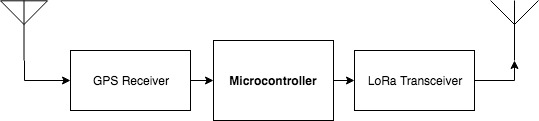
\includegraphics[width=12cm]{figures/node.jpeg}
    \caption{Node Diagram}
    \label{fig:node}
    \end{figure}

    A simple node was designed, built and programmed in C, consisting of an ESP8266 microcontroller, u-blox MAX8C GPS receiver and a Microchip RN2483 LoRa transceiver, as shown in figure \ref{fig:node}. The RN2483 was chosen as it implements the full LoRaWAN stack on-board, reducing the complexity of the microcontroller code. The GPS receiver used a basic chip antenna whilst the LoRA transceiver used an 868MHz 'rubber ducky' antenna. The specific hardware is not particularly important however, but rather the functionality is.

    The GPS receiver was configured to pedestrian mode since the primary method of testing would be a person walking with the node, as opposed to a flight or high velocity mode. The LoRaWAN configuration parameters (device address, network session key and application session key) were hard-coded into the microcontroller firmware.

    The microcontroller follows a basic loop. In each iteration, set at roughly every 10 seconds, the microcontroller requests data from the GPS (latitude, longitude, altitude, number of satellites and time) and loads it into a struct datatype. A counter in the microcontroller's flash memory, such that it is persistent across power cycling, is incremented and also added to the struct. The entire 20 byte struct is then transmitted as a binary blob payload by the LoRa transceiver. Other functionality allowing transmission on a button press and short bursts of continuous data transmission was also implemented but not ultimately used.

    The main file of the node firmware can be seen in appendix \ref{ap:nodefirmware}.


  \section{Server-side Software}

    \begin{figure}
    \centering
    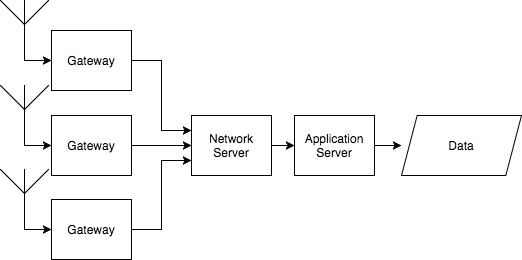
\includegraphics[width=12cm]{figures/server.jpeg}
    \caption{LoRaWAN to Server Diagram}
    \label{fig:server}
    \end{figure}

    When a gateway receives a packet from a node, it uploads it to the network server. The data can then be passed by the network server over an HTTP connection to the relevant application server, if the application server has implemented the necessary JSON-RPC methods \cite{EverynetAPI}. A python script to be run on a public server with open port 8080 is found in appendix \ref{ap:servereverynet} and implements the 'uplink' and 'post\_uplink' methods. The 'uplink' method provides data as soon as one gateway has received a packet whilst the 'post\_uplink' method should provide data on all receiving gateways a few seconds later. Unfortunately after testing, it was found that this latter method is not functional and that therefore obtaining details on all gateways is not possible this way. Hopefully it will be in the future.

    Therefore, a workaround was found by using the unofficial API running the Things Connected dashboard. The last 20 received packets from each gateway are available from a 'messages' endpoint. By continuously polling this endpoint at a rate faster than that at which the node is transmitting, all data from all gateways can be collected. Figure \ref{fig:server} shows a simplified system diagram for the LoRaWAN and server-side systems. A python script to perform an HTTP POST request to login and continually fetch data from the unofficial API through HTTP GET requests is found in appendix \ref{ap:serverfetch}. The fetched data is published to a Redis Pub/Sub channel which is subscribed to by another script, found in appendix \ref{ap:serverprocess}, where the data is processed. The payload of each packet is decoded and the binary blob unpacked into the constituent pieces of data. If the packet payload already exists in the Redis database, the details of the new gateway receiving the packet is appended to the gateway list. If it doesn't already exist, the entire packet data is freshly inserted into the database.

    It is at this point in the system that any final positioning algorithm would ultimately be included. Instead, another python script, in appendix \ref{ap:serverexport}, allows all the received data to be exported from the database to a JSON file for analysis and testing.



\chapter{Data Analysis \& Results}

  In this chapter, the gathered data and the various transformations, algorithms and analytics carried out will be presented alongside the final positioning errors obtained. All investigations were programmed in Python and carried out in an iPython Jupyter notebook.

  \section{Gathered Data}

    The GPS node was taken for a walk through central London, through both areas with a high number and low number of gateways. Table \ref{tab:gatewaynums} shows the number of gateways that each packet was received by, with 648 packets received in total by 8 different unique gateways. It can be seen that only about 25\% of packets were received by 3 or more gateways, with three gateways being the minimum requirement to estimate a 2-dimensional position.

    Figure \ref{fig:datamap} provides a geographical visualization of the data. The location of each gateway that received a packet is shown in blue, the true location of packets received by less than 3 gateways are shown in red and the true location of packets received by 3 or more gateways are shown in green. With a cursory glance, it can be seen that generally more packets are received by higher numbers of gateways in areas of high gateway density.

    Taking a closer look at the received data, each gateway provides the latitude, longitude and altitude of its position and a timestamp with microsecond precision. Since the position coordinates for each gateway vary between packets, it would seem that for every packet received, a new location is retrieved from the GPS. It is unknown whether the timestamp is also retrieved live from the GPS, or from an internal clock. Either way, microsecond precision is not ideal bearing in mind that \SI{1}{\micro\second} is equivalent to 300 metres in distance. This also means it is unlikely the timestamping occurs at the instant a packet is first received.

    \begin{table}[ht]
      \begin{center}
        \caption{Number of packets received by n gateways}
        \label{tab:gatewaynums}
        \begin{tabular}{|c|c|c|c|c|c|c|}
          \hline
          Number of Gateways & 1 & 2 & 3 & 4 & 5 & Total \\
          \hline
          Number of Packets & 310 & 168 & 111 & 46 & 13 & 648 \\
          \hline
        \end{tabular}
      \end{center}
    \end{table}

    \begin{figure}[ht]
    \centering
    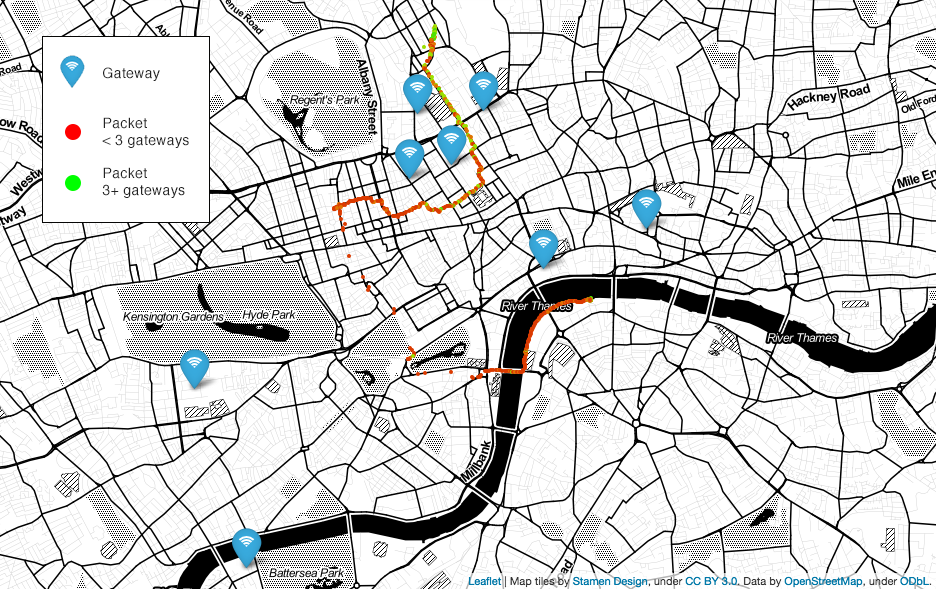
\includegraphics[width=15cm]{figures/map_data.png}
    \caption{Geographical visualization of gathered data}
    \label{fig:datamap}
    \end{figure}


  \section{Cartesian Coordinates}
    When working with the TDOA algorithms, it is important that a linear cartesian coordinate system is used, as opposed to the WGS84 latitude and longitude used by the GPS.

    If 3-dimensional positioning was required, latitude, longitude and altitude (LLA) could be converted to the Earth Centred, Earth Fixed (ECEF) frame and vice versa. In this reference frame, the origin is at the centre of the Earth with the x-axis intersecting the Greenwich meridian and the equator, the z-axis being along the spin axis of the Earth and the y-axis being perpendicular to both of these. However, for 3-dimensional position estimates, a minimum of 4 gateways would be required and the effect of altitude is likely to be negligible compared to other sources of error.

    For 2-dimensional positioning, a local grid reference frame can be used. Latitude and longitude can be converted to OSGB36, the British Ordnance Survey National Grid reference system, and vice versa, through a number of calculations and adjustments detailed in OSTN02 \cite{OSTN02}. The resulting cartesian coordinates are in metres and also allow for easy plotting of the hyperbolic equations and position estimates. When positioning errors and distances are given, it is simply the euclidean distance between two sets of (x,y) coordinates in metres.

  \section{Received Signal Strength}

    The Received Signal Strength Indicator (RSSI) has already been discounted as a viable method of positioning due to the broad number of factors involved of which distance is only one. Figure \ref{fig:rssidistance} plots the RSSI of each packet received by each gateway against the distance from the transmission to the gateway. Whilst it can be seen that there is a relationship, the large variance of RSSI for any distance, particularly at the lower end, makes it unusable for positioning on its own.

    \begin{figure}[ht]
    \centering
    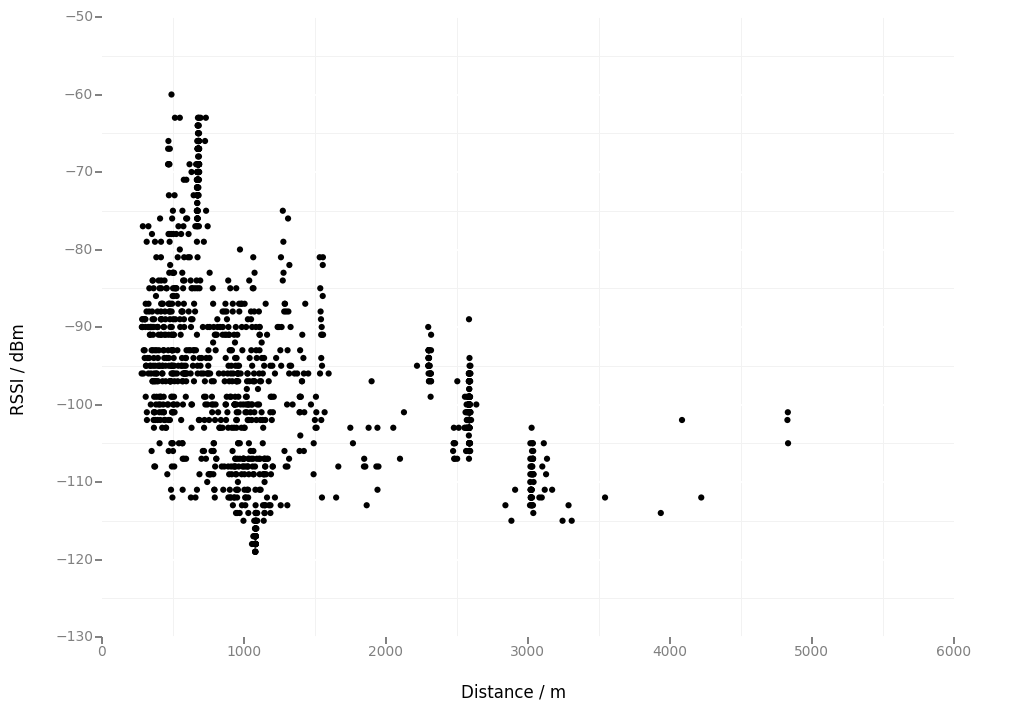
\includegraphics[width=15cm]{figures/rssidistance.png}
    \caption{Relationship between RSSI and distance from gateway}
    \label{fig:rssidistance}
    \end{figure}

  %\section{Data Cleanup}

  %  It was found after initial investigations and whilst programming Chan's algorithm that there were numerous issues with the data. The first issue is that some packets appeared to be received by one gateway more than once with varied receive times. Whether this is due to an issue with the particular gateway, or its location causing excessive multipath effects is unknown.

  \section{Chan's Algorithm}

    Initial investigations were carried out using an implementation of Chan's algorithm \cite{Chan1994}.

    The results of applying Chan's algorithm to the raw data directly, choosing the latter 3 gateways to have received each packet, were disappointing and can be seen in table \ref{tab:chanresults}. Out of 170 possible packets that were received by 3 or more gateways, the algorithm only returned position estimates for 18, or about 11\%. The mean positional error of these when compared to the true locations was 1112 metres.

    When the hyperbolic equations were plotted, it was found that the majority of packets did not have hyperbola that ever intersected or did not have hyperbola that were even valid due to the limited precision of the gateway timestamps. One such instance can seen in figure \ref{fig:hyperbolanointersect}. A limitation of Chan's algorithm is that it calculates exact solutions to the hyperbolic equations, so in all these instances where no exact solutions exist it was unable to provide a result.

    \begin{figure}[ht]
    \centering
    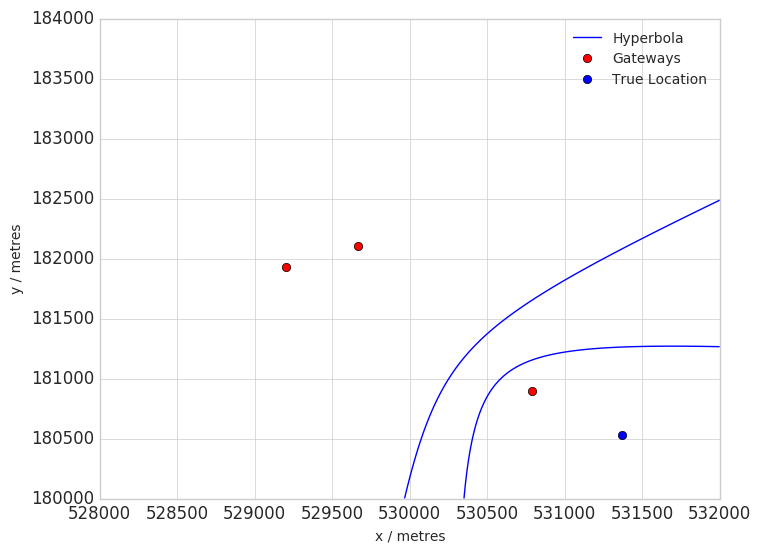
\includegraphics[width=10cm]{figures/hyperbolanointersect.png}
    \caption{Geographical plot of packet with non-intersecting hyperbola}
    \label{fig:hyperbolanointersect}
    \end{figure}

    \begin{table}[ht]
      \begin{center}
        \caption{Results of Chan's algorithm}
        \label{tab:chanresults}
        \begin{tabular}{|c|c|c|c|c|c|c|}
          \hline
           & Resolvable Packets & Mean Error & Median Error & Standard Deviation \\
          \hline
          Raw Data & 10.6\% & 1112m & 882m & 671m \\
          \hline
          Offsets & 17.0\% & 38,810m & 903m & 110,200m \\
          \hline
          Offsets (outliers removed) & 14.1\% & 866m & 642m & 767m \\
          \hline
        \end{tabular}
      \end{center}
    \end{table}

  \section{Offsets}

    In an attempt to improve the initial results achieved with Chan's algorithm, both in terms of the number of packets with a solution and in terms of the positional error, it was theorized that each gateway may have a timing offset associated with it which could be corrected for. Offsets cannot be calculated for each gateway individually since we are using TDOA and do not have an exact transmit time, but offsets for pairs of gateways can be found.

    The offset of a pair of gateways, i and j, is shown in equation \ref{eq:offset}. The result of the difference of the euclidean distances from the true position of the packet, \(d_i - d_j\), divided by the speed of light, C, is what the time difference of arrival should be. Therefore the difference of this value and the TDOA, \(t_i - t_j\), provides a time offset for that pair of gateways.

    \begin{equation}
    \label{eq:offset}
    offset_{ij} = (\frac{d_i - d_j}{C}) - (t_i - t_j)
    \end{equation}

    The offset is calculated for every possible pair of gateways for every packet. The probability density function (PDF) for these offsets is shown in figure \ref{fig:offsetpdf} and it can be seen that they are quite varied, with the majority of values within \SI{10}{\micro\second} and the mean at \SI{3.58}{\micro\second}. In terms of distance, that is a mean offset of over 1km.

    \begin{figure}[ht]
    \centering
    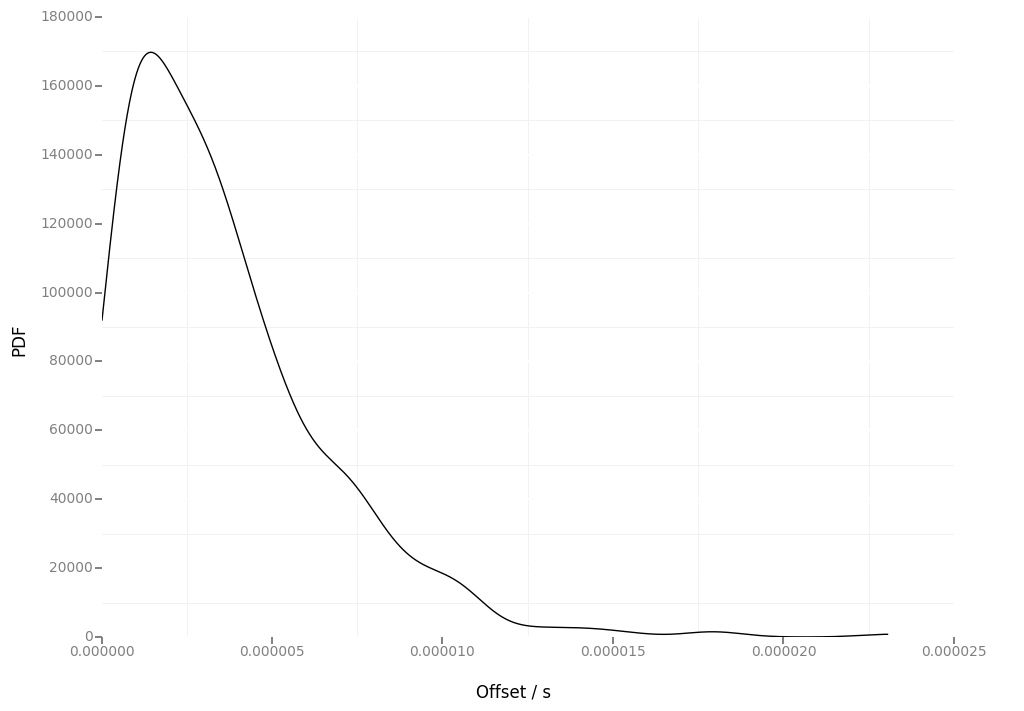
\includegraphics[width=12cm]{figures/offsetpdf.png}
    \caption{Probability Density Function for all calculated offsets}
    \label{fig:offsetpdf}
    \end{figure}

    \begin{figure}[ht]
    \centering
    \begin{subfigure}[b]{7cm}
        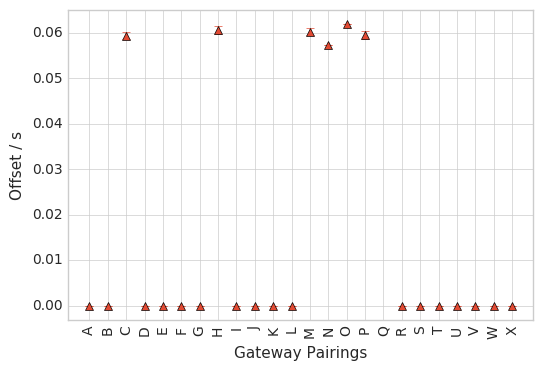
\includegraphics[height=5cm]{figures/offsetsall.png}
        \caption{All gateway pairs}
        \label{fig:offsetboxesa}
    \end{subfigure}
    ~
    \begin{subfigure}[b]{7cm}
        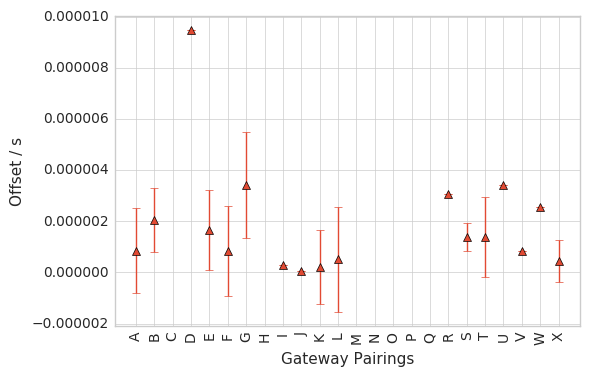
\includegraphics[height=5cm]{figures/offsetssmall.png}
        \caption{Gateway pairs with \si{\micro\second} offsets}
        \label{fig:offsetboxesb}
    \end{subfigure}
    \caption{Mean and Standard Deviations of Calculated Offsets} \label{fig:offsetboxes}
    \end{figure}

    Of greater significance are the spread of values for each individual pairing, shown in figures \ref{fig:offsetboxesa} and \ref{fig:offsetboxesb}. \ref{fig:offsetboxesa} shows that some pairings have mean offsets of as high as 0.06s, which would cause significant errors in positioning and likely cause no solution to be found at all. \ref{fig:offsetboxesb} narrows down to those pairings with offsets in the microsecond range and allows the standard deviation bars to be seen. These show that the offsets are not particularly constant for most pairings, perhaps suggesting that other factors are involved such as multipath and non-line-of-sight effects or just that the gateways do not assign a timestamp in a particularly controlled way.

    Applying these mean offsets to the TDOAs before using Chan's algorithm results in slight improvements with a solution for 17\% of packets, shown in row 2 of table \ref{tab:chanresults}. Due to clear outliers however, resulting in solutions tens of kilometres from the gateways, the mean positional error is almost 40km but with a median of only 903m. Removing these outliers gives solutions for about 14\% of packets with a mean positional error of 866m, shown in row 3 of table \ref{tab:chanresults}, down from an error of 1112m without applying offsets.


  \section{Iterative Algorithm}

    Even with the addition of offsets, Chan's algorithm severely limits the number of resolvable packets. Ideally an approximate solution is needed in the cases when the hyperbolic equations do not intersect and this is provided by utilizing an iterative algorithm rather than a closed. With the implementation of a least squares based iterative algorithm, an exact solution does not need to exist. In addition, all the data in over-determined situations can more easily be used, potentially improving the estimation accuracy - i.e. when there are more than 3 gateways that have received a packet and thus more TDOA equations than there are unknown coordinates. Being an iterative algorithm, an initial estimate is required and the further the estimate from the true solution, the more iterations it will take to converge on a solution. To keep processing times down, a limit on the number of iterations will normally be set and so ideally the initial estimate will be set to be as close to the solution as possible. With trial and error of several potential initial estimates, including using the origin (0,0) and the result of the previous estimate, it was found that using the position of the first receiving gateway minimized the number of packets which did not converge. The only other possible disadvantage of an iterative technique compared to a closed form algorithm such as Chan is the processing time - however, the processing is being performed on the server-side rather than an embedded device and so this an inconsequential issue.

    When the iterative algorithm was run on the raw data, the results were immediately an improvement with a solution returned for about 44\% of packets that were received by three or more gateways, compared to 14\% with reasonable error for Chan's algorithm. As shown in row 1 of table \ref{tab:iterresults}, the mean positional error achieved was 972m, a similar figure to Chan's.

    Since all receiving gateways are taken into account using the iterative algorithm, improvements were found by rejecting outliers in the receiving gateway timestamps. Erroneous times that would clearly put the node beyond the reach of the network were rejected, resulting in solutions for over 58\% of packets with a mean positional error of just over 1km, shown in row 2 of table \ref{tab:iterresults}. By also applying the offsets for gateway pairs before using the iterative algorithm, solutions were found for about 55\% of packets with a mean positional error of 930m and a lower standard deviation of 557m, shown in row 3 of table \ref{tab:iterresults}.

    \begin{table}[ht]
      \begin{center}
        \caption{Results of Iterative algorithm}
        \label{tab:iterresults}
        \begin{tabular}{|c|c|c|c|c|c|c|}
          \hline
           & Resolvable Packets & Mean Error & Median Error & Standard Deviation \\
          \hline
          Raw Data & 44.1\% & 972m & 850m & 614m \\
          \hline
          Raw Data (reject outliers) & 58.2\% & 1080m & 929m & 716m \\
          \hline
          Offsets & 55.3\% & 930m & 863m & 557m \\
          \hline
        \end{tabular}
      \end{center}
    \end{table}

    To better visualize the positional error, \ref{fig:iterrorpdf} plots the probability density function for the iterative algorithm with offsets applied. Whilst the mean error is just under 1km, the variability of the positional error is large with errors as great as 3km occurring. Precise and reliable positioning would therefore appear to be beyond the scope of the current network, but a rough position over a broad city scenario can certainly be achieved.

    \begin{figure}[ht]
    \centering
    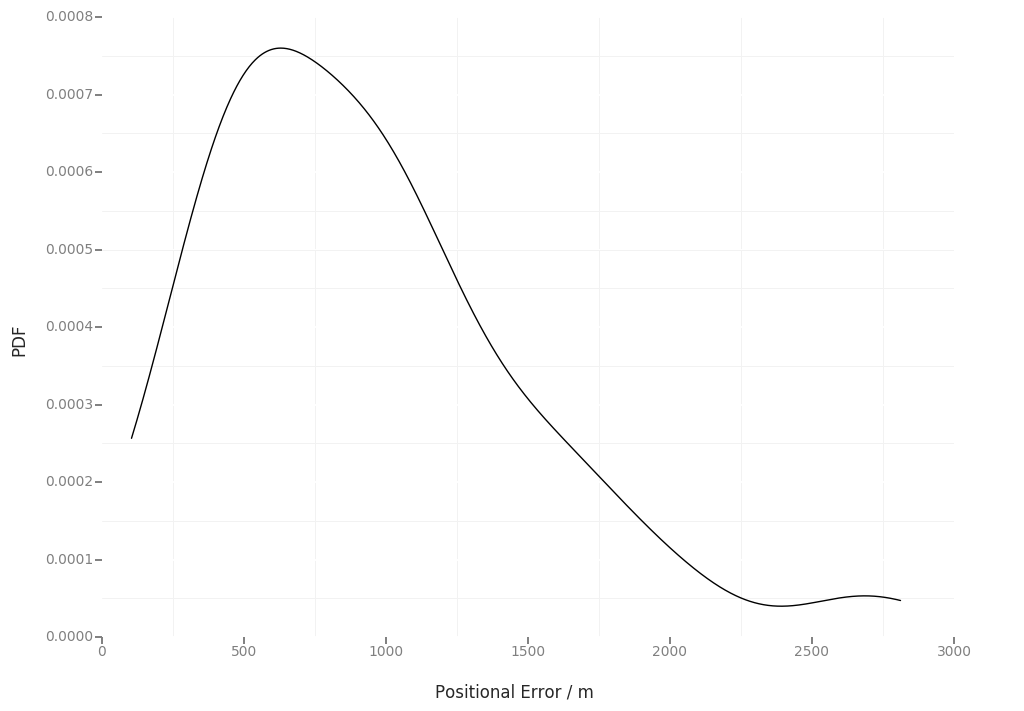
\includegraphics[width=12cm]{figures/iterativeoffseterrorpdf.png}
    \caption{Probability Density Function for Positional Error using Iterative Algorithm with Offsets}
    \label{fig:iterrorpdf}
    \end{figure}


  \section{Oversampling}

    Lastly, oversampling was employed in an attempt to improve the positional accuracy and reduce noise. With the test node stationary at one location known to be picked up by multiple gateways, a large number of transmissions were made. Two methods were considered to test the viability of oversampling, the first being to calculate every possible TDOA and find the mean for each gateway pair to achieve a higher resolution time difference. The second was to find an estimated location for every packet and take the mean of the coordinates as the final estimate. This latter method was chosen as simpler and likely to produce similar results.

    \begin{table}[ht]
      \begin{center}
        \caption{Results of Oversampling with Iterative algorithm}
        \label{tab:osresults}
        \begin{tabular}{|c|c|c|>{\bfseries}c|}
          \hline
           & Resolvable Packets & Mean Error &  Final Estimate Error \\
          \hline
          Data & 29\% & 1196m & 467m \\
          \hline
          Data (reject outliers) & 64\% & 1198m & 392m \\
          \hline
        \end{tabular}
      \end{center}
    \end{table}

    Running the iterative algorithm on each individual packet received from the location resulted in a mean positional error of almost 1.2km with only 29\% of packets achieving a solution. However, the mean location calculated from the set of estimated coordinates achieved a far lower positional error of just 467m, shown in row 1 of table \ref{tab:osresults}.

    Running the algorithm again whilst rejecting outliers resulted in a mean positional error of almost 1.2km but with 64\% of packets achieving a solution. With more packets therefore being using to estimate the final location, a positional error of 392m is found, shown in row 2 of table \ref{tab:osresults}. These results are visualized in figure \ref{fig:oversampleplot}, where the individual location estimates can be seen with the final estimated location in green and true location in blue.

    Whilst these results are promising and more accurate than estimating locations based on an individual transmission, this method is likely only suitable for use on stationary nodes. Whilst transmitting multiple packets in bursts is possible, it is undesirable both due to power constraints and sharing use of the network amongst potentially large numbers of other nodes. In reality, any oversampling of location will happen over longer periods of time, reducing usefulness for moving nodes which are the primary use case for positioning.

    \begin{figure}[ht]
    \centering
    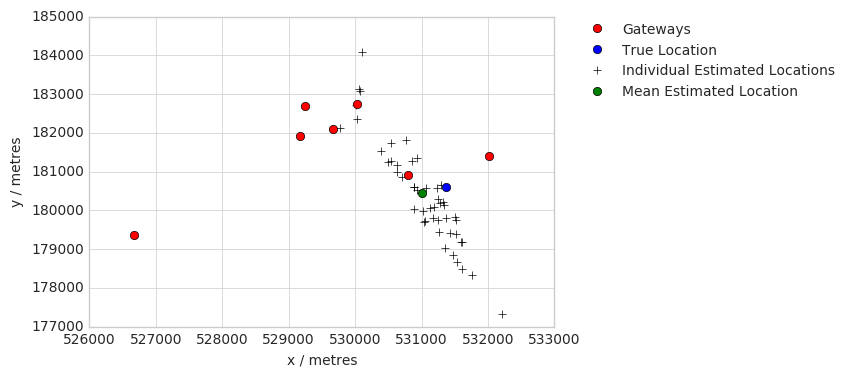
\includegraphics[width=16cm]{figures/oversampleplot.png}
    \caption{Geographical plot of oversampling with iterative algorithm}
    \label{fig:oversampleplot}
    \end{figure}





\chapter{Conclusion}

  Since only 50\% of packets were received by 3 or more gateways and a further x\% were rejected, leaving only y\% of packets with location estimates, it is clear that the LoRaWAN network used is not ideal for positioning. However, it is important to note this is a relatively new network and that with a broader spread of gateways, these numbers are likely to be greatly improved. It should also be noted that investigating the number of receiving gateways and distance from gateways was not a primary aim and ideally more data representing a greater geographical spread around the network's gateways would be collected and thus the reliability of these statistics improved.

  Ideally offsets need to be calculated on LOS only transmissions, in a large open space. Quantify the effects of NLOS/multipath. Also, cross validation should be performed with a larger dataset, else overfitting of offsets to dataset - particularly in case of gateway pairings with only a few transmissions, or even just one transmission, *optimistically biased*.

  Iterative algorithm better than closed form for such unreliable, unprecise data. Might be better algorithms than least squares though? Kalman?

  Indoor, short range, precise not possible with current hardware.

  Future: design own gateways with proper, accurate, precise timestamping! Gateways calculate offset from one another
  Combine RSSI and TDOA???   Machine learning due to noisy NLOS environment??

  MORE GATEWAYS, MORE WIDELY SPREAD - more chance of LOS / closer to LOS, and more 3+ gateways




% Example Chapter for Stuff
\chapter{Example Chapter}

  \section{Aims}
  I aim to do things, as shown in equation (\ref{eq:myeq}). I will show how to do this in Section \ref{app}.

  \begin{equation}
  \label{eq:myeq}
  f(x) = \dot{x} + B u(t) + C x(x)
  \end{equation}


  \section{Apparatus}
  \label{app}

  	50\% of my study.

      A diagram of how to set up the apparatus is shown in figure \ref{fig:app}.

      \begin{figure}
      \centering
      %\includegraphics[height=5cm]{blank}
      \caption{Apparatus setup}
      \label{fig:app}
      \end{figure}

  \section{Observations}

  %This was demonstrated in \cite{Bonfils2014}.

  \section{Discussion}

      These results can be seen in table \ref{fig:myt}.

      \begin{table}
      \begin{center}
      \caption{Predicted and measured beam deflections}
      \label{fig:myt}
      \begin{tabular}{|c|c|c|c|}
  	\hline
  	Thing & thing & thing & thing \\
  	\hline
  	Another & another & another & another \\
  	\hline
      \end{tabular}
      \end{center}

      \end{table}


% Bibliography
\bibliographystyle{unsrt}
\bibliography{references}

% Appendix
\appendix
\chapter{Node Firmware} \label{ap:nodefirmware}

\chapter{Server-Side Software}
  \section{Python Everynet API Script} \label{ap:servereverynet}
  \section{Python Fetch Script} \label{ap:serverfetch}
  \section{Python Processing Script} \label{ap:serverprocess}
  \section{Python Export Script} \label{ap:serverexport}


\end{document}
